
\graphicspath{{figures/complex/}}

%\setcounter{secnumdepth}{0}
%\renewcommand{\theequation}{\thechapter.\arabic{equation}}
%\renewcommand{\thetheorem}{\thechapter.\arabic{theorem}}
%\renewcommand{\thebc}{\thechapter.\arabic{theorem}}
%\renewcommand{\theeg}{\thechapter.\arabic{theorem}}
%\counterwithin{theorem}{chapter}
%\numberwithin{theorem}{chapter}

\chapter{Complex Numbers and Exponentials}\label{ap:complex}
 
%%%%%%%%%%%%%%%%%%%%%%%%%%%%%%%%%%%%%%%%%%%%%%%%%%%%%%%
\section{Definition and Basic Operations}\label{sec complex defn}
%%%%%%%%%%%%%%%%%%%%%%%%%%%%%%%%%%%%%%%%%%%%%%%%%%%%%%%
We'll start with the definition of a complex number and its addition and multiplication rules. You may find the multiplication rule quite mysterious. Don't worry. We'll soon gets lots of practice using it 
and seeing how useful it is.
\begin{defn}\label{def complex}
\begin{enumerate}[(a)]
\item
The complex plane is simply the $xy$-plane equipped with an addition operation and a multiplication operation.
A complex number is nothing more than a point in that $xy$-plane.
 It is conventional to use the notation $x+iy$\footnote{In electrical engineering it is conventional to use $x+jy$ instead of $x+iy$.}
to stand for the complex number $(x,y)$. In other words, it is conventional
to write $x$ in place of $(x,0)$ and $i$ in place of $(0,1)$.
\item
 The first component, $x$, of the complex number $x+iy$
is called its real part and the second component, $y$, is called its 
imaginary part, even though there is nothing imaginary\footnote{Don't 
attempt to attribute any special significance to the word ``complex'' in 
``complex number'', or to the word ``real'' in ``real number'' and 
``real part'', or to the word ``imaginary'' in ``imaginary part''. 
All are {\it just names}.
The name ``imaginary'' was introduced by Ren\'e Descartes in 1637. 
Ren\'e Descartes (1596--1650) was a French scientist and philosopher, who 
lived in the Dutch Republic for roughly twenty years after serving in the 
(mercenary) Dutch States Army. Originally, ``imaginary'' was a derogatory term and imaginary numbers were thought to be useless. But they turned out to be incredibly useful!}
 about it.
\item
The sum of the complex numbers $\, z_1=x_1+i y_1 $ and $\, z_2=x_2 +iy_2 \, $ is defined by
\begin{equation*}
z_1+z_2 = (x_1+x_2)+i(y_1+y_2)
\end{equation*}
That is, you just separately add the real parts and the imaginary parts.
\end{enumerate}
\end{defn}

\addtocounter{theorem}{-1}
\begin{defn}[continued]
\begin{enumerate}[(a)]
\item[(d)]
The product of the complex numbers $\, z_1=x_1+i y_1 $ and
$\, z_2=x_2 +iy_2 \, $ is defined by
\begin{equation*}
z_1z_2 = x_1x_2-y_1y_2+i(x_1y_2+x_2y_1)
\end{equation*}
Do not memorise this multiplication rule. We'll see a simple, effective memory aid for it shortly.
The heart of that memory aid is the observation that the complex number $i$ has the special property that
\begin{equation*}
i^2 = (0+1i)(0+1i) = (0\times 0-1\times 1)+i(0\times 1+1\times 0) = -1
\end{equation*}
\end{enumerate}
\end{defn}
Addition and multiplication of complex numbers obey the familiar addition rules
\begin{align*}
z_1+z_2&=z_2+z_1  \\
z_1+(z_2+z_3)&=(z_1+z_2)+z_3 \\
0+z_1&=z_1 
\end{align*}
and multiplication rules
\begin{align*}
z_1z_2&=z_2z_1 \\
z_1(z_2z_3)&=(z_1z_2)z_3 \\
1z_1&=z_1 
\end{align*}
and distributive laws
\begin{align*}
z_1(z_2+z_3)&=z_1z_2+z_1z_3 \\
(z_1+z_2)z_3& = z_1z_3+z_2z_3 
\end{align*}
To remember how to multiply complex numbers, you just have to supplement
the familiar rules of the real number system with $i^2=-1$. The previous 
sentence is the memory aid referred to in  Definition~\ref{def complex}(d). 
\begin{eg}\label{eg add multiply}
If $z=1+2i$ and $w=3+4i$, then
\begin{alignat*}{3}
z+w&=(1+2i)+(3+4i)&&=4+6i \\
zw&=(1+2i)(3+4i)&&=3+4i+6i+8i^2=3+4i+6i-8=-5+10i
\end{alignat*}
\end{eg}
\begin{defn}\label{def add mult inverse}
\begin{enumerate}[(a)]
\item
The negative of any complex number $z= x+iy$ is defined by 
\begin{equation*}
-z=-x+(-y)i
\end{equation*}
and obviously obeys $z+(-z)=0$.
\item
The reciprocal\footnote{The reciprocal $z^{-1}$ is also called the multiplicative inverse of $z$.}, $z^{-1}$ or $\frac{1}{z}$, of any complex 
number $z= x+iy$, other than $0$, is defined by 
\begin{equation*}
\frac{1}{z}z =1
\end{equation*}
We shall see below that it is given by the formula
 \begin{equation*}
z^{-1}=\frac{1}{z}=\frac{x}{x^2+y^2}+\frac{-y}{x^2+y^2}i
\end{equation*}
\end{enumerate}
\end{defn}
\begin{eg}\label{eg mult inverse}
It is possible to derive the formula for $\frac{1}{z}$ by observing that
\begin{equation*}
(a+ib)(x+iy)=[ax-by] + i[ay+bx]
\end{equation*} 
equals $1 = 1+i0$ if and only if
\begin{align*}
ax-by&=1 \\
ay+bx&=0
\end{align*}
and solving these equations for $a$ and $b$. We will see a much shorter 
derivation in Remark~\ref{rem inverse} below. For now, we'll content 
ourselves with just verifying that $\frac{x}{x^2+y^2}+\frac{-y}{x^2+y^2}i$ 
is the inverse of $x+iy$ by multiplying out
\begin{align*}
\left(\frac{x}{x^2+y^2}-\frac{y}{x^2+y^2}i\right)(x+iy)
&=\frac{x^2}{x^2+y^2}-\frac{xy}{x^2+y^2}i
+\frac{xy}{x^2+y^2}i-\frac{y^2}{x^2+y^2}i^2 \\
&=\frac{x^2-i^2y^2}{x^2+y^2}
=\frac{x^2+y^2}{x^2+y^2}=1
\end{align*}
%The formula $\frac{1}{x+iy}=\frac{x}{x^2+y^2}-\frac{y}{x^2+y^2}i$ is
%not as mysterious as it looks. 
\end{eg}
\begin{defn}\label{def conjugate}
\begin{enumerate}[(a)]
\item
The complex conjugate of $\, z=x+iy\, $ is denoted $\bar z$ and is
defined to be 
\begin{equation*}
\bar z=\overline{x+iy}=x-i y
\end{equation*} 
That is, to take the complex conjugate, one
replaces every $i$ by $-i$ and vice versa.
\item
The distance from $z=x+iy$ (recall that this is the point $(x,y)$ in the 
$xy$-plane) to $0$ is  denoted $\, |z|\, $ and is called the
absolute value, or modulus,  of $\, z\, $.  It is given by
\begin{equation*}
|z| = \sqrt{x^2+y^2}
\end{equation*}
Note that 
\begin{equation*}
z\bar z=(x+iy)(x-iy)=x^2-ixy+ixy+y^2=x^2+y^2
\end{equation*}
is always a nonnegative real number and that
\begin{equation*}
|z| = \sqrt{z\,\bar z}
\end{equation*}
\end{enumerate}
\end{defn}
\begin{remark}\label{rem inverse}
Let $z=x+iy$ with $x$ and $y$ real. Since $|z|^2=z\,\bar z$, we have
\begin{align*}
\frac{1}{z} =\frac{1}{z}\frac{\bar z}{\bar z} = \frac{\bar z}{|z|^2} =\frac{x-iy}{x^2+y^2}
=\frac{x}{x^2+y^2}+\frac{-y}{x^2+y^2}i
\end{align*}
which is the formula for $\frac{1}{z}$ given in 
Definition~\ref{def add mult inverse}(b).
\end{remark}
\begin{eg}\label{eg:division}
It is easy to divide a complex number by a real number. For example
\begin{equation*}
\frac{11+2i}{25} = \frac{11}{25}+\frac{2}{25}i
\end{equation*}
In general, the complex conjugate provides us with a trick for rewriting 
any ratio of complex numbers as a ratio with a real denominator. 
For example, suppose that we want to find $\frac{1+2i}{3+4i}$. The trick is 
to multiply by $1=\frac{3-4i}{3-4i}$. The number $3-4i$ is the complex conjugate of the denominator $3+4i$. Since $(3+4i)(3-4i)=9-12i+12i-16i^2=9+16=25$
\begin{equation*}
\frac{1+2i}{3+4i}=\frac{1+2i}{3+4i}\ \frac{3-4i}{3-4i}
=\frac{(1+2i)(3-4i)}{25}
=\frac{11+2i}{25}
= \frac{11}{25}+\frac{2}{25}i
\end{equation*}
\end{eg}
\begin{defn}\label{def Re Im}
The notations\footnote{The symbols $\Re$ and $\Im$ are the letters $R$ and $I$
in the Fraktur font, which was created in the early 1500's and became common in the German-speaking world. A standard alternative notation is $\text{Re}(z)$ 
and $\text{Im}(z)$.} $\Re z$ and $\Im z$ stand for the real and imaginary parts 
of the complex number $z$, respectively. If $z=x+ iy$ (with $x$ and $y$ real) 
they are defined by 
\begin{equation*}
\Re z=x\qquad \Im z=y
\end{equation*}
Note that both $\Re z$ and $\Im z$ are real numbers.
Just subbing in  $\bar z=x-iy$, you can verify that
\begin{equation*}
\Re z=\frac{1}{2}(z+\bar z)\qquad \Im z=\frac{1}{2i}(z-\bar z)
\end{equation*}
\end{defn}
\begin{lemma}\label{lem mod prod}
If $z_1=x_1+iy_1$ and $z_2=x_2+iy_2$, then
\begin{equation*}
|z_1z_2| = |z_1|\,|z_2|
\end{equation*}
\end{lemma}
\begin{proof}
Since $z_1z_2=(x_1+iy_1)(x_2+iy_2)=(x_1x_2-y_1y_2)+i(x_1y_2+x_2y_1)$,
\begin{align*}
|z_1z_2| &=\sqrt{(x_1x_2-y_1y_2)^2+(x_1y_2+x_2y_1)^2} \\
 &=\sqrt{x_1^2x_2^2-\textcolor{blue}{2x_1x_2y_1y_2}+y_1^2y_2^2
+x_1^2y_2^2+\textcolor{blue}{2x_1y_2x_2y_1}+x_2^2y_1^2} \\
 &=\sqrt{x_1^2x_2^2+y_1^2y_2^2+x_1^2y_2^2+x_2^2y_1^2} 
=\sqrt{(x_1^2+y_1^2)(x_2^2+y_2^2)} \\
 &=|z_1|\,|z_2| 
\end{align*}
\end{proof}


%%%%%%%%%%%%%%%%%%%%%%%%%%%%%%%%%%%%%%%%%%%%%%%%%%%%%%%
\section{The Complex Exponential}\label{sec complex exp}
%%%%%%%%%%%%%%%%%%%%%%%%%%%%%%%%%%%%%%%%%%%%%%%%%%%%%%%
\subsection{Definition and Basic Properties.}\label{ssec complex exp def}
%%%%%%%%%
There are two equivalent standard definitions of the exponential, $e^z$,
of the complex number $z=x+iy$. For the more intuitive definition, one simply 
replaces the real number $x$ in the Taylor series expansion\footnote{See Theorem~\ref{thm:SRimportantTaylorSeries}.}
$e^x=\sum_{n=0}^\infty \frac{x^n}{n!}$ with the complex number $z$, giving
\begin{equation*}
e^z=\sum_{n=0}^\infty \frac{z^n}{n!}
\tag{EZ}\end{equation*}
 We instead highlight the more computationally useful definition. 
\begin{defn}\label{def complex exp}
For any complex number $z=x+iy$, with $x$ and $y$ real, the exponential 
$\, e^z\, $, is defined by
\begin{equation*}
e^{x+iy}\ =\ e^x\cos y+i e^x\sin y
\end{equation*}
In particular\footnote{The equation $e^{iy}\ =\ \cos y+i \sin y$ is known as Euler's formula. Leonhard Euler (1707--1783) was a  Swiss mathematician and physicist who spent most of his adult life in Saint Petersberg and Berlin. He gave the name $\pi$ to the ratio of a circle's circumference to its diameter. He also developed the constant $e$. His collected works fill 92 volumes.}, $e^{iy}\ =\ \cos y+i \sin y$.
\end{defn}
We will not fully prove that the intuitive definition (EZ) and the computational
Definition~\ref{def complex exp} are equivalent. But we will do so in the special case that $z=iy$, with $y$ real. Under (EZ),
\begin{equation*}
e^{iy} = 1 +iy +\frac{(iy)^2}{2!}+\frac{(iy)^3}{3!}+\frac{(iy)^4}{4!}
+\frac{(iy)^5}{5!}+\frac{(iy)^6}{6!}+\cdots
\end{equation*}
The even terms in this expansion are
\begin{equation*}
1  +\frac{(iy)^2}{2!}+\frac{(iy)^4}{4!}+\frac{(iy)^6}{6!}+\cdots
=1  -\frac{y^2}{2!}+\frac{y^4}{4!}-\frac{y^6}{6!}+\cdots
=\cos y
\end{equation*}
and the odd terms in this expansion are
\begin{equation*}
 iy +\frac{(iy)^3}{3!}+\frac{(iy)^5}{5!}+\cdots
=i\Big(y-\frac{y^3}{3!}+\frac{y^5}{5!}+\cdots\Big)
=i\sin y
\end{equation*}
Adding the even and odd terms together gives us that, under (EZ), $e^{iy}$ is indeed equal to $\cos y + i\sin y$.\footnote{It is obvious that, in the special case that $z=x$ with $x$ real, the definitions (EZ) and \ref{def complex exp} are equivalent. So to complete the proof of equivalence in the general case $z=x+iy$, it suffices to prove that $e^{x+iy}=e^x e^{iy}$ under both (EZ) and 
Definition~\ref{def complex exp}. For Definition~\ref{def complex exp}, this follows from Lemma \ref{lem_exp_ppties}, below.} As a consequence, we have
\begin{equation*}
e^{i\pi}=-1
\end{equation*}
which gives an amazing linking between calculus ($e$), geometry ($\pi$),
algebra ($i$) and the basic number $-1$.

In the next lemma we verify that the complex exponential obeys a couple of familiar computational properties.
\begin{lemma}\label{lem_exp_ppties}
\begin{enumerate}[(a)]
\item 
For any complex numbers $z_1$ and $z_2$,
\begin{equation*}
e^{z_1+z_2} = e^{z_1}e^{z_2}
\end{equation*}
\item
For any complex number $c$,
\begin{equation*}
\diff{}{t}e^{ct} = c e^{ct}
\end{equation*}
\end{enumerate}
\end{lemma}
\begin{proof}
\begin{enumerate}[(a)]
\item
For any two complex numbers $z_1=x_1+iy_1$ and $z_2=x_2+iy_2$,
with $x_1$, $y_1$, $x_2$, $y_2$ real,
\begin{align*}
e^{z_1}e^{z_2}
&= e^{x_1}(\cos y_1+i \sin y_1)e^{x_2}(\cos y_2+i \sin y_2) \\
&= e^{x_1+x_2}(\cos y_1+i \sin y_1)(\cos y_2+i \sin y_2) \\
&= e^{x_1+x_2}\left\{(\cos y_1\cos y_2-\sin y_1\sin y_2)
              +i (\cos y_1\sin y_2+\cos y_2\sin y_1)\right\} \\
&= e^{x_1+x_2}\left\{\cos(y_1+y_2)+i\sin(y_1+y_2)\right\} \\
&\hskip1in\text{by the trig identities of Appendix~\ref{sec trig add}} \\
&= e^{(x_1+x_2)+i(y_1+y_2)} \\
&= e^{z_1+z_2}
\end{align*}
so that the familiar multiplication formula also applies to complex exponentials.

\item
For any real number $t$ and any complex number $c=\alpha+i\beta$, 
with $\alpha$, $\beta$ real,
\begin{equation*}
e^{ct}=e^{\alpha t+i\beta t}=e^{\alpha t}[\cos( \beta t)+i\sin(\beta t)]
\end{equation*}
so that the derivative with respect to $t$ 
\begin{align*}
\diff{}{t} e^{ct}
&=\alpha e^{\alpha t}[\cos( \beta t)+i\sin(\beta t)]
   +e^{\alpha t}[-\beta\sin( \beta t)+i\beta \cos(\beta t)] \\
&=(\alpha+i\beta) e^{\alpha t}[\cos( \beta t)+i\sin(\beta t)] \\
&=ce^{ct}
\end{align*}
is also the familiar one.
\end{enumerate}
\end{proof} 
%%%%%%%%%%
\subsection{Relationship with $\sin$ and $\cos$.}\label{ssec complex sin cos}
%%%%%%%%%
\begin{impeqn}\label{eqn euler}
When $\theta$ is a real number
\begin{align*}
e^{i \theta} &= \cos \theta+i \sin \theta \\
e^{-i \theta} &= \cos \theta-i \sin \theta=\overline{e^{i\theta}}
\end{align*}
are complex numbers of modulus one.
\end{impeqn}
Solving for $\cos\theta$ and $\sin\theta$ (by adding and subtracting the two equations) gives
\begin{impeqn}\label{eqn exp sin cos}
\begin{alignat*}{3}
\cos\theta&=\frac{1}{2}(e^{i\theta}+e^{-i\theta})&&=\Re e^{i\theta} \\
\sin\theta&=\frac{1}{2i}(e^{i\theta}-e^{-i\theta})&&=\Im e^{i\theta}
\end{alignat*}
\end{impeqn}
 
\begin{eg}\label{eg complex trig id}
These formulae make it easy derive trig identities. For example,
\begin{align*}
\cos\theta\cos\phi &= \frac{1}{4}\big(e^{i\theta}+e^{-i\theta}\big)
                                 \big(e^{i\phi}+e^{-i\phi}\big) \\
 &= \frac{1}{4}\big(e^{i(\theta+\phi)}+e^{i(\theta-\phi)}
                    +e^{i(-\theta+\phi)}+e^{-i(\theta+\phi)}\big) \\
&= \frac{1}{4}\big(e^{i(\theta+\phi)}+e^{-i(\theta+\phi)}
           +e^{i(\theta-\phi)} +e^{i(-\theta+\phi)}\big) \\
&= \frac{1}{2}\big(\cos(\theta+\phi)+\cos(\theta-\phi)\big)
\end{align*}
and, using $(a+b)^3=a^3+3a^2b+3ab^2+b^3$,
\begin{align*}
\sin^3\theta&=-\frac{1}{8i}\big(e^{i\theta}-e^{-i\theta}\big)^3\cr
&=-\frac{1}{8i}\big(e^{i3\theta}-3e^{i\theta}
                +3e^{-i\theta}-e^{-i3\theta}\big) \\
&=\frac{3}{4}\frac{1}{2i}\big(e^{i\theta}-e^{-i\theta}\big)
-\frac{1}{4}\frac{1}{2i}\big(e^{i3\theta}-e^{-i3\theta}\big) \\
&=\frac{3}{4}\sin\theta-\frac{1}{4}\sin(3\theta)
\end{align*}
and
\begin{align*}
\cos(2\theta)&=\Re\big(e^{2\theta i}\big)=\Re \big(e^{i\theta}\big)^2 \\
&=\Re \big(\cos \theta+i\sin\theta\big)^2 \\
&=\Re \big(\cos^2 \theta+2i\sin\theta\cos\theta-\sin^2\theta\big) \\
&=\cos^2\theta-\sin^2\theta
\end{align*}
\end{eg}
%%%%%%%%%%
\subsection{Polar Coordinates.}\label{ssec complex polar}
%%%%%%%%%
Let $z=x+iy$ be any complex number. Writing $x$ and $y$ in polar coordinates
in the usual way, i.e. $x=r\cos(\theta)$, $y=r\sin(\theta)$,  gives
\begin{align*}
x+iy=r\cos\theta+ir\sin\theta=re^{i\theta}\qquad
\end{align*}
See the figure on the left below. In particular
\begin{alignat*}{5}
1  &=\ \ \ \  e^{i0}      &&= e^{2\pi i}         &&= e^{2k\pi i}             
          &&\quad\text{for }k=0,\pm 1,\pm2,\cdots \\
-1 &=\ \ \  e^{i\pi}    &&= e^{3\pi i}         &&= e^{(1+2k)\pi i}         
          &&\quad\text{for }k=0,\pm 1,\pm2,\cdots \\
i  &=\   e^{i\pi/2}  &&= e^{{5\over 2}\pi i} &&= e^{({1\over 2}+2k)\pi i}
          &&\quad\text{for }k=0,\pm 1,\pm2,\cdots \\
-i &=  e^{-i\pi/2} &&=e^{{3\over 2}\pi i}  &&= e^{(-{1\over 2}+2k)\pi i}
          &&\quad\text{for }k=0,\pm 1,\pm2,\cdots 
\end{alignat*}
See the figure on the right below.
\begin{efig}
\begin{center}
   \raisebox{0.23\height}{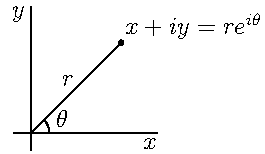
\includegraphics{polar}}\qquad 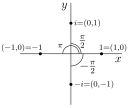
\includegraphics{polar2}
\end{center}
\end{efig}
The polar coordinate $\theta=\arctan\frac{y}{x}$ associated with the
complex number $z=x+iy$, i.e. the point $(x,y)$ in the $xy$-plane,
is also called the argument of $z$.

The polar coordinate representation makes it easy to find square roots,
third roots and so on. Fix any positive integer $n$. The $n^{\rm th}$ roots
of unity are, by definition, all solutions $z$ of
\begin{equation*}
z^n\ =\ 1
\end{equation*}
Writing $z=re^{i\theta}$
\begin{equation*}
r^ne^{n\theta i}\ =\ 1e^{0i}
\end{equation*}
The polar coordinates $(r,\theta)$ and $(r',\theta')$ represent the same point
in the $xy$-plane if and only if $r=r'$ and $\theta=\theta'+2k\pi$ for some
integer $k$. So $z^n=1$ if and only if $r^n=1$, i.e. $r=1$, and 
$n\theta =2 k\pi$ for some integer $k$. The $n^{\rm th}$ roots of unity are 
all the complex numbers $e^{2\pi i{k\over n}}$ with $k$ integer. There are 
precisely $n$ distinct $n^{\rm th}$ roots of unity because 
$e^{2\pi i{k\over n}}=e^{2\pi i{k'\over n}}$ if and only if 
$2\pi {k\over n}-2\pi {k'\over n}=2\pi {k-k'\over n}$ is
an integer multiple of $2\pi$. That is, if and only if $k-k'$ is an integer
multiple of $n$. The $\, n\, $ distinct $n^{\rm th}$ roots of unity are
\begin{equation*}
1\ ,\ e^{2\pi i{1\over n}}\ ,\ e^{2\pi i{2\over n}}
\ ,\  e^{2\pi i{3\over n}}\ ,\ \cdots\ ,\ e^{2\pi i{n-1\over n}}
\end{equation*}
For example, the $6^{\rm th}$ roots of unity are depicted below.
\begin{efig}
\begin{center}
   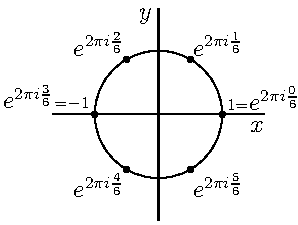
\includegraphics{polar3}
\end{center}
\end{efig}


%%%%%%%%%%
\subsection{Exploiting Complex Exponentials in Calculus Computations}
       \label{ssec complex calculus}
%%%%%%%%%

You have learned how to evaluate integrals involving trigonometric functions
by using integration by parts, various trigonometric identities and various
substitutions. It is often much easier to just use (\ref{eqn euler}) and
(\ref{eqn exp sin cos}). Part of the utility of complex numbers comes from 
how well they interact with calculus through the exponential function.
Here are two examples
\begin{eg}\label{eg complex calc A}
\begin{align*}
\int e^x\cos x\ \dee{x}&=\frac{1}{2} \int e^x\big[e^{ix}+e^{-ix}\big]\ \dee{x}
=\frac{1}{2}  \int \big[e^{(1+i)x}+e^{(1-i)x}\big]\ \dee{x} \\
&=\frac{1}{2}  \left[\frac{1}{1+i}e^{(1+i)x}+\frac{1}{1-i}e^{(1-i)x}\right]+C
\end{align*}
This form of the indefinite integral looks a little weird because of
the $i$'s. While it looks complex because of the $i$'s, it is actually purely real (and correct), because $\frac{1}{1-i}e^{(1-i)x}$ is the complex conjugate 
of $\frac{1}{1+i}e^{(1+i)x}$. We can convert the indefinite integral into
a more familiar form just by subbing back in $e^{\pm ix}=\cos x\pm i\sin x$,
$\frac{1}{1+i}=\frac{1-i}{(1+i)(1-i)}=\frac{1-i}{2}$ and
$\frac{1}{1-i}=\overline{\frac{1}{1+i}}=\frac{1+i}{2}$. 
\begin{align*}
\int e^x\cos x\ \dee{x}
&=\frac{1}{2}  e^x\left[\frac{1}{1+i}e^{ix}+\frac{1}{1-i}e^{-ix}\right]+C\\
&=\frac{1}{2}  e^x\left[\frac{1-i}{2}(\cos x+i\sin x)
   +\frac{1+i}{2}(\cos x-i\sin x)\right]+C \\
&=\frac{1}{2}  e^x\cos x+\frac{1}{2} e^x\sin x+C
\end{align*}
You can quickly verify this by differentiating (or by comparing with 
Example~\ref{eg:PRTSexsinx}).
\end{eg}

\begin{eg}\label{eg complex calc B}
Evaluating the integral $\int\cos^nx\ \dee{x}$ using the methods of Section~\ref{sec trigint} can be a real pain. It is much easier if we convert
to complex exponentials. Using $(a+b)^4=a^4+4a^3b+6a^2b^2+4ab^3+b^4$,
\begin{align*}
\int \cos^4 x\ \dee{x}&=\frac{1}{2^4} \int\big[e^{ix}+e^{-ix}\big]^4\ \dee{x}
=\frac{1}{2^4} \int \big[e^{4ix}+4e^{2ix}+6+4e^{-2ix}+e^{-4ix}\big]\ \dee{x} \\
&=\frac{1}{2^4} \left[\frac{1}{4i}e^{4ix}+\frac{4}{2i}e^{2ix}+6x
+\frac{4}{-2i}e^{-2ix}+\frac{1}{-4i}e^{-4ix}\right]+C\cr
&=\frac{1}{2^4} \left[\frac{1}{2}\frac{1}{2i}(e^{4ix}-e^{-4ix})
              +\frac{4}{2i}(e^{2ix}-e^{-2ix})+6x\right]+C\cr
&=\frac{1}{2^4} \left[\frac{1}{2}\sin 4x+4\sin 2x+6x\right]+C \\
&=\frac{1}{32} \sin 4x+\frac{1}{4}\sin 2x+\frac{3}{8}x+C
\end{align*}
\end{eg}

%%%%%%%%%%%%%%%%%%%%%%%%%%%%%%%%%%%
\begin{comment}
Complex numbers can also be used to simplify partial fraction computations.
Here is an example

\begin{eg}\label{eg complex calc C}
In this example, we shall find $\int \frac{x+2}{x^2+2x+5}\ \dee{x}$.
Using complex numbers, any polynomial can be written as a product of linear
factors. This allows us to eliminate quadratic denominators from the partial
fractions procedure. This example illustrates how.
\begin{itemize}
\item
We first have to factor the denominator $x^2+2x+5$. We can use the
high school formula for the solutions of the quadratic equation
$x^2+2x+5=0$:
\begin{equation*}
\frac{-2\pm\sqrt{2^2-4\times 5}}{2}=\frac{-2\pm\sqrt{4-20}}{2}
=-1\pm\sqrt{-4}=-1\pm 2i
\end{equation*}
Or we can complete the square
\begin{align*}
x^2+2x+5&=(x+1)^2+4=(x+1)^2-(2i)^2=[(x+1)-2i][(x+1)+2i] \\
&=[x+1-2i][x+1+2i]
\end{align*}
\item
Next we write the integrand in the form
\begin{equation*}
\frac{x+2}{x^2+2x+5}
=\frac{x+2}{(x+1-2i)(x+1+2i)}
=\frac{a}{x+1-2i}+\frac{b}{x+1+2i}
\end{equation*}
with the constants $a$ and $b$ chosen so that
\begin{equation*}
\frac{a}{x+1-2i}+\frac{b}{x+1+2i}
=\frac{a(x+1+2i)+b(x+1-2i)}{(x+1-2i)(x+1+2i)}
=\frac{x+2}{(x+1-2i)(x+1+2i)}
\end{equation*}
i.e. so that 
\begin{equation*}
a(x+1+2i)+b(x+1-2i)=x+2
\end{equation*}
This has to be true for all $x$. We can solve easily for $a$ if we choose
$x+1=2i$ (so that the coefficient of $b$ is zero) and we can solve easily 
for $b$ if we choose $x+1=-2i$ (so that the coefficient of $a$ is zero):
\begin{align*}
x+1&=2i & &\Rightarrow &
          a(2i+2i)+b(2i-2i)&=2i+1 \\ 
        && &\Rightarrow &
          4i\,a&=1+2i \\
        && &\Rightarrow &
           a&=\frac{1+2i}{4i}=\frac{1}{2}-\frac{1}{4}i \\
x+1&=-2i & &\Rightarrow &
          a(-2i+2i)+b(-2i-2i)&=-2i+1  \\
        && &\Rightarrow &
          -4i\,b&=1-2i \\ 
        && &\Rightarrow &
          b&=-\frac{1-2i}{4i}=\frac{1}{2}+\frac{1}{4}i
\end{align*}
since $\frac{1}{i}=-i$.
As a check, we observe that, with $a=\frac{1}{2}-\frac{1}{4}i$ and  
$b=\frac{1}{2}+\frac{1}{4}i$,
\begin{align*}
a(x+1+2i)+b(x+1-2i)
&= \left(\frac{1}{2}-\frac{1}{4}i\right)(x+1+2i)+
   \left(\frac{1}{2}+\frac{1}{4}i\right)(x+1-2i) \\
&=(x+1) \left(\frac{1}{2}-\frac{1}{4}i+\frac{1}{2}+\frac{1}{4}i\right)+
    2i\left(\frac{1}{2}-\frac{1}{4}i-\frac{1}{2}-\frac{1}{4}i\right) \\
&=x+1+2i\left(-\frac{1}{2}i\right)=x+2
\end{align*}
as desired.
\item
 The integral is now easy,
\begin{align*}
\int \frac{x+2}{x^2+2x+5}\ \dee{x}
&=\int\left[\frac{a}{x+1-2i}+\frac{b}{x+1+2i}\right]\ \dee{x} \\
&=a\log(x+1-2i)+b\log(x+1+2i)+C \\
&=\left(\frac{1}{2}-\frac{1}{4}i\right)\log(x+1-2i)
           +\left(\frac{1}{2}+\frac{1}{4}i\right)\log(x+1+2i)+C
\end{align*}
though the answer looks a little wierd because of the complex numbers and also
because \textbf{we don't yet know what the definition of $\log(z)$ is when $z$ is complex}. 
\item
One can eliminate the complex numbers by using the fact that, 
for $X$ and $Y$ real numbers,
\begin{equation*}
\log(X\pm iY)=\log\sqrt{X^2+Y^2}\pm i\tan^{-1}\frac{Y}{X}
\tag{L}\end{equation*}
To derive (L), write $\log(X\pm iY)=U\pm iV$, with $U$ and $V$ real. 
Then $U$ and $V$ are to be determined by $e^{U\pm iV}=X\pm iY$ or
$e^U\big(\cos V\pm i\sin V)=X\pm iY$ or 
\begin{equation*}
e^U\cos V=X\qquad e^U\sin V=Y
\end{equation*}
Dividing the last two equations gives $\tan V=\frac{Y}{X}$ and adding
the squares of the last two equations together gives $e^{2U}=X^2+Y^2$.
\item
Applying (L) with $X=x+1$ and $Y=2$ gives
\begin{align*}
&\left(\frac{1}{2}-\frac{1}{4}i\right)\log(x+1-2i)
+\left(\frac{1}{2}+\frac{1}{4}i\right)\log(x+1+2i) \\
&\hskip1in=\left(\frac{1}{2}-\frac{1}{4}i\right)
              \left(\log\sqrt{x^2+2x+5}-i\tan^{-1}\frac{2}{x+1}\right) \\
&\hskip1.5in+\left(\frac{1}{2}+\frac{1}{4}i\right)
              \left(\log\sqrt{x^2+2x+5}+i\tan^{-1}\frac{2}{x+1}\right) \\
&\hskip1in=\log\sqrt{x^2+2x+5}-\frac{1}{2} \tan^{-1}\frac{2}{x+1}
\end{align*}
\end{itemize}

\end{eg}
\end{comment}

%%%%%%%%%%
\subsection{Exploiting Complex Exponentials in Differential Equation Computations}       \label{ssec complex de}
%%%%%%%%%
 
Complex exponentials are also widely used to simplify the process
of guessing solutions to ordinary differential equations. We'll start with
(possibly a review of) some basic definitions and facts about
differential equations.

\begin{defn}\label{def:apODE}
\begin{enumerate}[(a)]
\item %%% (a)
A \emph{differential equation} is an equation for an
unknown function that contains the derivatives of that unknown function.
For example $y''(t)+y(t)=0$ is a differential equation for the unknown 
function $y(t)$.

\item %% (b) 
In the differential calculus text CLP-1, we treated only derivatives of functions of one variable. Such derivatives are called ordinary derivatives. 
A differential equation is called an \emph{ordinary differential
equation} (often shortened to ``ODE'') if only ordinary derivatives 
appear. That is, if the unknown function has only a single independent
variable. 

In CLP-3 we will treat derivatives of functions of more than one variable.
For example, let $f(x,y)$ be a function of two variables. If you treat $y$ as a constant and take the derivative of the resulting function of the single variable $x$, the result is called the partial derivative of $f$ with 
respect to $x$. A differential equation is called a \emph{partial differential
equation} (often shortened to ``PDE'') if partial derivatives
appear. That is, if the unknown function has more than one independent
variable. For example $y''(t)+y(t)=0$ is an ODE while
$\frac{\partial^2 u}{\partial\, t^2}(x,t)=c^2 
\frac{\partial^2 u}{\partial\, x^2}(x,t)$ is a PDE.

\item %% (c) 
The \emph{order} of a differential equation is the order of the
highest derivative that appears. For example $y''(t)+y(t)=0$ 
is a second order ODE.

\item %% (d) 
An ordinary differential equation that is of the form
\begin{equation}\label{eqn:ODEordern}
a_0(t) y^{(n)}(t) + a_1(t) y^{(n-1)}(t)+\cdots+a_{n-1}(t) y'(t) +a_n(t)y(t)
=F(t)
\end{equation}
with given coefficient functions $a_0(t)$, $\cdots$, $a_n(t)$ and $F(t)$ 
is said to be \emph{linear}. Otherwise, the ODE is said to be \emph{nonlinear}.
For example, $y'(t)^2+y(t)=0$, $y'(t)y''(t)+y(t)=0$ and $y'(t)=e^{y(t)}$
are all nonlinear.

\item %% (e) 
The ODE \eqref{eqn:ODEordern} is said to have \emph{constant coefficients} if
the coefficients  $a_0(t)$, $a_1(t)$, $\cdots$, $a_n(t)$ are all constants. Otherwise,
it is said to have \emph{variable coefficients}. For example,
the ODE $y''(t)+7y(t)=\sin t$ is constant coefficient, while 
$y''(t)+ty(t)=\sin t$ is variable coefficient.

\item[(f)] %% (f) 
The ODE \eqref{eqn:ODEordern} is said to be \emph{homogeneous} if $F(t)$ 
is identically zero. Otherwise, it is said to be \emph{inhomogeneous} or 
\emph{nonhomogeneous}. For example, the ODE $y''(t)+7y(t)=0$ is homogeneous, 
while  $y''(t)+7y(t)=\sin t$ is inhomogeneous. A homogeneous ODE always
has the trivial solution $y(t)=0$.

\end{enumerate}
\end{defn}

\addtocounter{theorem}{-1}
\begin{defn}[continued]
\begin{enumerate}[(a)]

\item[(g)] %% (g) 
An \emph{initial value problem}  is a problem in which one is to find
an unknown function $y(t)$ that satisfies both a given ODE and given
initial conditions, like $y(t_0)=1$, $y'(t_0)=0$. Note that all of the 
conditions involve the function $y(t)$ (or its derivatives) evaluated at 
a single time $t=t_0$.

\item[(h)] %% (h) 
A \emph{boundary value problem}  is a problem in which one is to find
an unknown function $y(t)$ that satisfies both a given ODE and given
boundary conditions, like $y(t_0)=0$, $y(t_1)=0$. Note that the conditions 
involve the function $y(t)$ (or its derivatives) evaluated at two different 
times. 

\end{enumerate}
\end{defn}


\noindent The following theorem gives the form of solutions to the 
linear\footnote{There are a some special classes of nonlinear ODE's, like the separable differential equations of \S\ref{sec sep de}, that are relatively easy to solve. But generally, nonlinear ODE's are much harder to solve than linear ODE's.} ODE \eqref{eqn:ODEordern}.

\begin{theorem}\label{thm:odeMain}
Assume that the coefficients $a_0(t)$, $a_1(t)$, $\cdots$, $a_{n-1}(t)$, 
$a_n(t)$ and $F(t)$ are continuous functions and that 
$a_0(t)$ is not zero.

\begin{enumerate}[(a)]
\item %% (a) 
The general solution to the linear ODE \eqref{eqn:ODEordern} is of the form
\begin{equation}\label{eqn:ODEgensln}
y(t)=y_p(t)+ C_1y_1(t)+C_2y_2(t)+\cdots+C_n y_n(t)
\end{equation}
where 
\begin{itemize}\itemsep1pt \parskip0pt \parsep0pt %\itemindent-15pt
\item[$\circ$] $n$ is the order of \eqref{eqn:ODEordern}
\item[$\circ$] $y_p(t)$ is \textbf{any} solution to \eqref{eqn:ODEordern}
\item[$\circ$] $C_1$, $C_2$, $\cdots$, $C_n$ are arbitrary constants
\item[$\circ$] $y_1$, $y_2$, $\cdots$, $y_n$ are $n$ independent solutions
to the homogenous equation 
\begin{equation*}
a_0(t) y^{(n)}(t) + a_1(t) y^{(n-1)}(t)+\cdots+a_{n-1}(t) y'(t) +a_n(t)y(t)=0
\end{equation*}
associated to \eqref{eqn:ODEordern}.
``Independent'' just means that no $y_i$ can be written as a linear combination
of the other $y_j$'s. For example, $y_1(t)$ cannot be expressed in the form
$b_2y_2(t)+\cdots+b_ny_n(t)$. 
\end{itemize}
In \eqref{eqn:ODEgensln}, $y_p$ is called the ``particular solution'' and 
$C_1y_1(t)+C_2y_2(t)+\cdots+C_n y_n(t)$ is called the 
``complementary solution''.

\item %% (b) 
Given any constants $b_0$, $\cdots$, $b_{n-1}$ there is exactly
one function $y(t)$ that obeys the ODE \eqref{eqn:ODEordern} and the initial
conditions
\begin{equation*}
y(0)=b_0\qquad y'(0)=b_1\qquad \cdots\qquad y^{(n-1)}(0)=b_{n-1}
\end{equation*}
\end{enumerate}
\end{theorem}


In the following example we'll derive one widely used linear constant coefficient ODE.

\begin{eg}[RLC circuit]\label{eg:RLC}
As an example of how ODE's arise, we consider the RLC circuit, which is
the electrical circuit consisting of a resistor of
resistance $R$, a coil (or solenoid) of inductance $L$, a capacitor 
of capacitance $C$ and a voltage source arranged in series, as shown below. 
Here $R$, $L$
and $C$ are all nonnegative constants.
\begin{efig}
\begin{center}
    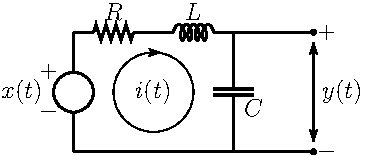
\includegraphics[scale=1.3]{RLC.pdf}
\end{center}
\end{efig}
 We're going to think of the voltage $x(t)$ as an input signal,
and the voltage $y(t)$ as an output signal. 
The goal is to determine the output signal produced by a given input signal. 
If $i(t)$ is the current flowing at time $t$ in the loop as shown and 
$q(t)$ is the charge on the capacitor, then the voltages across $R$, $L$ 
and $C$, respectively, at time $t$ are
$Ri(t)$, $L\diff{i}{t}(t)$ and $y(t)=\frac{q(t)}{C}$. By the Kirchhoff's 
law\footnote{Gustav Robert Kirchhoff (1824--1887) was a German physicist.
There are several sets of Kirchhoff's laws that are named after him ---
Kirchhoff's circuit laws, that we are using in this example, Krichhoff's
spectroscopy laws and Kirchhoff's law of thermochemistry. Kirchhoff and his collaborator Robert Bunsen, of Bunsen burner fame, invented the spectroscope.
%He also coined the term ``black-body radiation''.
} 
that says that the voltage between any two points has to be independent 
of the path used to travel between the two points, these three voltages 
must add up to $x(t)$ so that
\begin{equation}\label{eqn:RLCrlc}
Ri(t) + L\diff{i}{t}(t) + \frac{q(t)}{C} = x(t)
\end{equation}
Assuming that $R,\ L,\ C$ and $x(t)$ are known, this is still one 
differential equation in two unknowns, the current $i(t)$ and the charge $q(t)$. 
Fortunately, there is a relationship between the two. Because the current entering the capacitor is the rate of change of the charge on the capacitor
\begin{equation}\label{eqn:RLCiq}
i(t)=\diff{q}{t}(t) = Cy'(t)
\end{equation}
This just says that the capacitor cannot create or destroy charge on 
its own; all charging of the capacitor must come from the current.  
Substituting \eqref{eqn:RLCiq} into \eqref{eqn:RLCrlc} gives
\begin{equation*}%\label{eqn:RLCxyode}
 LCy''(t) + RCy'(t) + y(t) = x(t)
\end{equation*}
which is a second order linear constant coefficient ODE. 
As a concrete example, we'll take  an ac voltage source and choose the 
origin of time so that $x(0)=0$, $x(t)=E_0\sin(\omega t)$. Then the differential equation becomes
\refstepcounter{equation}\label{eqn:ODERy}
\begin{equation}\tag{\ref{eqn:ODERy}}
LCy''(t)+RCy'(t)+y(t)=E_0\sin(\omega t)
\end{equation}
\end{eg} 

Finally, here are two examples in which we use complex exponentials to solve an ODE.

\begin{eg}\label{eg complex ode A}
By Theorem~\ref{thm:odeMain}(a), the general solution to the ordinary differential equation
\begin{equation*}
y''(t)+4y'(t)+5y(t)=0
\tag{ODE}
\end{equation*}
is of the form $C_1 u_1(t)+C_2 u_2(t)$ with $u_1(t)$ and $u_2(t)$ being
two (independent) solutions to (ODE) and with $C_1$ and $C_2$
being arbitrary constants. The easiest way to find
$u_1(t)$ and $u_2(t)$ is to guess them. And the easiest way to guess them
is to try\footnote{The reason that $y(t)=e^{rt}$ is a good guess
is that, with this guess, all of $y(t)$, $y'(t)$ and $y''(t)$ are constants
times $e^{rt}$. So the left hand side of the differential equation is
also a constant, that depends on $r$, times $e^{rt}$. So we just have to
choose $r$ so that the constant is zero.} 
$y(t)=e^{rt}$, with $r$ being a constant to be determined.
Substituting $y(t)=e^{rt}$ into (ODE) gives
\begin{align*}
r^2 e^{rt} +4re^{rt}+5e^{rt}=0
\iff\big(r^2 +4r+5\big)e^{rt}=0
\iff r^2 +4r+5=0
\end{align*}
This quadratic equation for $r$ can be solved either by using the high
school formula or by completing the square.
\begin{align*}
r^2 +4r+5=0
&\iff (r+2)^2+1=0
\iff (r+2)^2=-1
\iff r+2=\pm i \\
&\iff r=-2\pm i
\end{align*}
So the general solution to (ODE) is
\begin{align*}
y(t)=C_1e^{(-2+i)t} + C_2e^{(-2-i)t}
\end{align*}
This is one way to write the general solution, but there are many others.
In particular there are quite a few people in the world who are (foolishly)
afraid\footnote{Embracing the complexity leads to simplicity.} of complex exponentials. We can hide them by using (\ref{eqn euler}) and
(\ref{eqn exp sin cos}).
\begin{align*}
y(t)&=C_1e^{(-2+i)t} + C_2e^{(-2-i)t}
     =C_1e^{-2t}e^{it} + C_2 e^{-2t}e^{-it} \\
     &=C_1e^{-2t}\big(\cos t+i\sin t \big) 
       +C_2 e^{-2t}\big(\cos t-i\sin t \big) \\
     &=(C_1+C_2) e^{-2t} \cos t 
       +(iC_1-iC_2) e^{-2t}\sin t \\
     &=D_1 e^{-2t} \cos t 
       +D_2 e^{-2t}\sin t 
\end{align*}
with $D_1=C_1+C_2$ and $D_2=iC_1-iC_2$ being two other arbitrary constants.
Don't make the mistake of thinking that $D_2$ must be complex because 
$i$ appears in the formula $D_2=iC_1-iC_2$ relating $D_2$ and $C_1,C_2$. 
No one said that $C_1$ and $C_2$ are real numbers. In fact, 
in typical applications, the arbitrary constants are determined by 
initial conditions and often $D_1$ and $D_2$ turn out to be real and 
$C_1$ and $C_2$ turn out to be complex. 
For example, the initial conditions  $y(0)=0$, $y'(0)=2$ force
\begin{align*}
0&=y(0) = C_1 + C_2
\cr
2&=y'(0) = (-2+i)C_1 + (-2-i)C_2
\end{align*}
The first equation gives $C_2=-C_1$ and then the second equation gives
\begin{align*}
(-2+i)C_1 - (-2-i)C_1 = 2
\iff 2iC_1=2
\iff iC_1=1
\iff C_1=-i,\ C_2=i
\end{align*}
and
\begin{align*}
D_1=C_1+C_2=0\qquad
D_2=iC_1-iC_2=2
\end{align*}
\end{eg}

\begin{eg}\label{eg complex ode B}
We shall now guess one solution (i.e. a particular solution)
to the differential equation
\begin{equation*}
y''(t)+2y'(t)+3y(t)=\cos t
\tag{ODE1}\end{equation*}
Equations like this arise, for example, in the  study of the RLC circuit.
We shall simplify the computation by exploiting that $\cos t=\Re e^{it}$.
First, we shall guess a function $Y(t)$ obeying 
\begin{equation*}
Y''+2Y'+3Y=e^{i t}
\tag{ODE2}\end{equation*}
Then, taking complex conjugates,
\begin{equation*}
\bar Y''+2\bar Y'+3\bar Y=e^{-i t}
\tag{$\overline{\text{ODE2}}$}\end{equation*}
and, adding $\frac{1}{2}$(ODE2) and $\frac{1}{2}$($\overline{\text{ODE2}}$) together will
give 
\begin{equation*}
(\Re Y)''+2(\Re Y)'+3(\Re Y)=\Re e^{i t}=\cos t
\end{equation*}
which shows that $\Re Y(t)$ is a solution to (ODE1).
Let's try $Y(t)=Ae^{i t}$, with $A$ a constant to be determined. This is a solution of (ODE2) if and only if
\begin{align*}
& & \difftwo{}{t}\big(Ae^{it}\big)
    +2\diff{}{t}\big(Ae^{it}\big)
    +3Ae^{it}&=e^{it} \\
&\iff& (i^2+2i+3)Ae^{it}&=e^{it} \\
&\iff& A&=\frac{1}{2+2i} 
\end{align*}
So $\frac{e^{it}}{2+2i}$ is a solution to (ODE2) and $\Re \frac{e^{it}}{2+2i}$ 
is a solution to (ODE1). To simplify this, write $2+2i$ in polar coordinates.
From the sketch
\begin{efig}
\begin{center}
   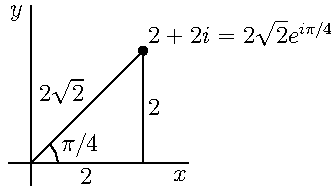
\includegraphics{polar4}
\end{center}
\end{efig}
we have $2+2i=2\sqrt{2}e^{i{\pi\over 4}}$.
So
\begin{align*}
\frac{e^{it}}{2+2i}&=\frac{e^{it}}{2\sqrt{2}e^{i{\pi\over 4}}}
=\frac{1}{2\sqrt{2}}e^{i(t-{\pi\over 4})} \\
\implies \Re\frac{e^{it}}{2+2i}
&=\frac{1}{2\sqrt{2}}\Re e^{i(t-{\pi\over 4})}
=\frac{1}{2\sqrt{2}}\cos\left(t-\frac{\pi}{4}\right)
\end{align*}
\end{eg}








